%\setchapterimage{bandeau}
\chapter*{TD \arabic{cptTD} \\ 
Gyrolock  \ifnormal $\star$ \else \fi \ifdifficile $\star\star$ \else \fi \iftdifficile $\star\star\star$ \else \fi
-- \ifprof Corrigé \else Sujet \fi}
\addcontentsline{toc}{section}{TD \arabic{cptTD} : 
Gyrolock \ifnormal $\star$ \else \fi \ifdifficile $\star\star$ \else \fi \iftdifficile $\star\star\star$ \else \fi
-- \ifprof Corrigé \else Sujet \fi}

\iflivret \stepcounter{cptTD} \else
\ifprof  \stepcounter{cptTD} \else \fi
\fi

\setcounter{question}{0}
\marginnote{Centrale Supelec PSI 2022.}
\marginnote[1cm]{
\UPSTIcompetence[2]{C1-05}
\UPSTIcompetence[2]{C2-09}
}

\ifprof  \marginnote{Corrigé proposé par l'UPSTI.}\else \fi

\subsection{\label{sec:II.C} Comportement dynamique du stabilisateur}

\begin{figure}[!h]
\centering
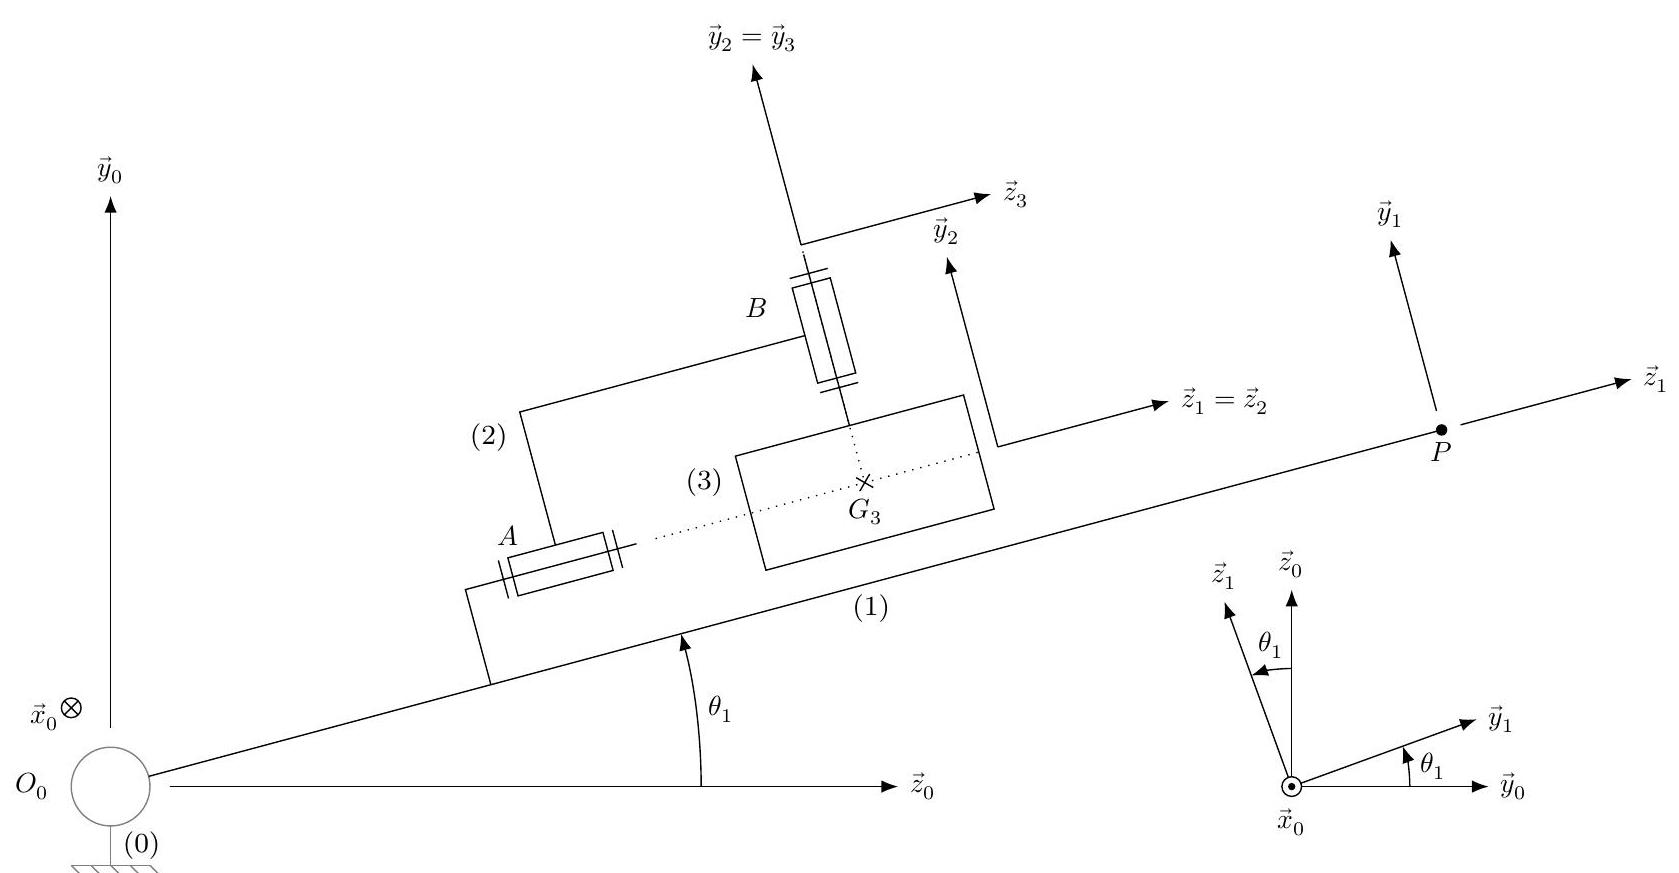
\includegraphics[width=\textwidth]{2023_07_26_54f5e859400a10e656ddg-06}
%Figure 9 
\caption{\label{fig:09}Modèle cinématique du système GyroLock (représenté pour $\theta_{2}=\theta_{3}=0$)}
\end{figure}

Dans la modélisation retenue (figure \ref{fig:09}), une liaison pivot non parfaite permet de représenter la flexibilité de l'attache reconfigurable. La table d'opération (0) est supposée fixe et le référentiel $\mathcal{R}_{0}\left(O_{0}, \vec{x}_{0}, \vec{y}_{0}, \vec{z}_{0}\right)$ lié à la table (0) est galiléen. Au stabilisateur (1) est associé le repère $\mathcal{R}_{1}\left(O_{0}, \vec{x}_{0}=\vec{x}_{1}, \vec{y}_{1}, \vec{z}_{1}\right)$ avec $\theta_{1}=\left(\vec{y}_{0}, \vec{y}_{1}\right)=\left(\vec{z}_{0}, \vec{z}_{1}\right)$. Le point $P$ tel que $O_{0} P=L$ représente le bout du stabilisateur (1) en contact avec la zone à opérer.

\subsection*{Paramétrage, notations et hypothèses}
\begin{itemize}
  \item La liaison pivot d'axe $\left(O_{0}, \vec{x}_{0}\right)$ entre les solides (0) et (1) possède une raideur $k$ et un coefficient de frottement visqueux $f$, d'où $\vec{M}\left(O_{0}, 0 \rightarrow 1\right) \cdot \vec{x}_{0}=-\left(k \theta_{1}+f \dot{\theta}_{1}\right)$;

  \item les autres liaisons sont supposées parfaites ;

  \item l'action du cœur sur le stabilisateur (1) est modélisée par $\left\{\mathcal{T}_{c \rightarrow 1}\right\}=\left\{\begin{array}{c}f_{c} \vec{y}_{1} \\ \overrightarrow{0}\end{array}\right\}_{P}$;

\item seul le déplacement vertical du point $P$ est pris en compte. On note $y(t)=-\overrightarrow{O_{0} P} \cdot \vec{y}_{0}$;

\item  le stabilisateur (1) est de masse $m_{1}$ et possède un centre d'inertie $G_{1}$ tel que $\overrightarrow{O_{0} G_{1}}=L_{G_{1}} \vec{z}_{1}$ et l'opérateur d'inertie est $\mathcal{J}\left(G_{1}, 1\right)=\left[\begin{array}{ccc}A_{1} & 0 & 0 \\ 0 & A_{1} & 0 \\ 0 & 0 & C_{1}\end{array}\right]_{\mathcal{B}_{1}} ;$

  \item la masse et l'inertie de l'étrier (2) sont négligeables ;

  \item la toupie (3) est de masse $m_{3}$ et possède un centre d'inertie $G_{3}$ tel que $\overrightarrow{O_{0} G_{3}}=L_{G_{3}} \vec{z}_{1}+H_{G_{3}} \vec{y}_{1}$;

  \item les figures de changement de base sont données figures 6 et 9 ;

  \item les actions mécaniques dues à la pesanteur sont négligées devant les effets dynamiques. Q 14. Sans détailler les calculs, donner la méthode permettant de déterminer la loi de mouvement du stabilisateur (équation différentielle en $\theta_{1}(t)$ ). L'ensemble isolé, l'inventaire des actions mécaniques extérieures, le théorème utilisé et sa projection scalaire sont à préciser clairement.

\end{itemize}

%Q 15. 
\question{\label{q:15}Exprimer $\vec{\delta}\left(O_{0}, 1 / 0\right) \cdot \vec{x}_{0}$, la projection sur $\vec{x}_{0}$ du moment dynamique au point $O_{0}$ du solide (1) en mouvement dans le référentiel $\mathcal{R}_{0}$.}
\ifprof
\begin{corrige}
Par formule de Varignon:

$$ \overrightarrow{\delta}(O_0,1/0)\cdot \overrightarrow{x}_0 = \overrightarrow{\delta}(G_1,1/0)\cdot \overrightarrow{x}_0 + \left( \overrightarrow{O_0 G_1} \wedge m_1 \overrightarrow{\Gamma}(G_1,1/0) \right)\cdot \overrightarrow{x}_0 $$

avec $\overrightarrow{\Gamma}(G_1,1/0) = \left. \dfrac{\mathrm{d}^2\overrightarrow{O_0 G_1}}{\mathrm{d}t^2} \right|_0 = -L_{G_1}\ddot{\theta}_1 \overrightarrow{y}_1 -L_{G_1}\dot{\theta}_1^2\overrightarrow{z_1}$ donc $\left( \overrightarrow{O_0 G_1} \wedge m_1 \overrightarrow{\Gamma}(G_1,1/0) \right)\cdot \overrightarrow{x}_0 = m_1 L_{G_1}^2\ddot{\theta}_1$.

De plus \textbf{au centre d'inertie} $G_1$: $\overrightarrow{\delta}(G_1,1/0)\cdot \overrightarrow{x}_0 = \left. \dfrac{\mathrm{d}\overrightarrow{\sigma}(G_1,1/0)\cdot \overrightarrow{x}_0}{\mathrm{d}t} \right|_0$ avec 

$\overrightarrow{\sigma}(G_1,1/0)\cdot \overrightarrow{x}_0 = \mathcal{I}(G_1,1)\overrightarrow{\Omega}(1/0)\cdot \overrightarrow{x}_0$.\\

Donc $\overrightarrow{\sigma}(G_1,1/0)\cdot \overrightarrow{x}_0 = A_1 \dot{\theta}_1$ et $\overrightarrow{\delta}(G_1,1/0)\cdot \overrightarrow{x}_0 = A_1 \ddot{\theta}_1$.\\

Finalement $\boxed{\overrightarrow{\delta}(O_0,1/0)\cdot \overrightarrow{x}_0 = (A_1 + m_1 L_{G_1}^2)\ddot{\theta}_1}$.

\end{corrige}
\else
\fi

%Q 16. 
\question{\label{q:16}Exprimer littéralement la vitesse $\vec{V}\left(G_{3}, 3 / 0\right)$ dans la base $\mathcal{B}_{1}$, puis l'accélération $\vec{\Gamma}\left(G_{3}, 3 / 0\right)$ dans la base $\mathcal{B}_{1}$.}
\ifprof
\begin{corrige}
Le point $G_3$ étant \textbf{physiquement rattaché à (3)} on peut écrire 

$\boxed{\overrightarrow{V}(G_3,3/0) = \left. \dfrac{\mathrm{d}\overrightarrow{O_0 G_3}}{\mathrm{d}t} \right|_0 = -L_{G_3}\dot{\theta}_1\overrightarrow{y}_1 + H_{G_3}\dot{\theta}_1\overrightarrow{z}_1}$.\\

Ensuite $\boxed{\overrightarrow{\Gamma}(G_3,3/0) = \left. \dfrac{\mathrm{d}\overrightarrow{V}(G_3,3/0)}{\mathrm{d}t} \right|_0 = -\left(L_{G_3}\ddot{\theta}_1 + H_{G_3}\dot{\theta}_1^2\right)\overrightarrow{y}_1 + \left(H_{G_3}\ddot{\theta}_1 - L_{G_3}\dot{\theta}_1^2\right)\overrightarrow{z}_1}$.

\end{corrige}
\else
\fi

%Q 17. 
\question{\label{q:17}En conservant les conditions de fonctionnement issues de la partie \ref{sec:II.A} $\left(\ddot{\theta}_{2} \approx 0, \theta_{2} \approx 0\right.$ et $\dot{\theta}_{3}=\omega_{3}$ constante), il est possible de montrer que $\vec{\delta}\left(G_{3}, 3 / 0\right) \cdot \vec{x}_{0}=A_{3} \ddot{\theta}_{1}-c_{x}(t)$ avec $c_{x}(t)=B_{3} \omega_{3} \dot{\theta}_{2}$ (résultat admis sans démonstration). En déduire $\vec{\delta}\left(O_{0}, 3 / 0\right) \cdot \vec{x}_{0}$, en fonction de $A_{3}, c_{x}(t), m_{3}, L_{G_{3}}, H_{G_{3}}$ et $\ddot{\theta}_{1}(t)$.}
\ifprof
\begin{corrige}
Par formule de Varignon:

\begin{align*}
\overrightarrow{\delta}(O_0,3/0)\cdot \overrightarrow{x}_0 &= \overrightarrow{\delta}(G_3,3/0)\cdot \overrightarrow{x}_0 + \left( \overrightarrow{O_0 G_3} \wedge m_3\overrightarrow{\Gamma}(G_3,3/0) \right)\cdot \overrightarrow{x}_0 \\
&= A_3 \ddot{\theta}_1 - c_x(t) +m_3L_{G_3}\left(L_{G_3}\ddot{\theta}_1 + H_{G_3}\dot{\theta}_1^2\right) + m_3 H_{G_3}\left(H_{G_3}\ddot{\theta}_1 - L_{G_3}\dot{\theta}_1^2\right)\\
&= \left(A_3 +m_3L_{G_3}^2 +m_3H_{G_3}^2\right) \ddot{\theta}_1 - c_x(t)
\end{align*}
 

\end{corrige}
\else
\fi

%Q 18. 
\question{\label{q:18}Exprimer $J_{x}$ en fonction de $A_{1}, A_{3}, m_{1}, m_{3}, L_{G_{1}}, L_{G_{3}}$ et $H_{G_{3}}$ permettant d'écrire la loi de mouvement du stabilisateur (1) sous la forme suivante :}
$$
J_{x} \ddot{\theta}_{1}(t)+f \dot{\theta}_{1}(t)+k \theta_{1}(t)=c_{x}(t)-L f_{c}(t)
$$
\ifprof
\begin{corrige}
En appliquant la stratégie vue en question 14 on a l'équation (effets dynamiques de (2) négligés et actions de la pesanteur négligées):

$$ \overrightarrow{\delta}(O_0,1/0)\cdot \overrightarrow{x}_0 + \overrightarrow{\delta}(O_0,3/0)\cdot \overrightarrow{x}_0 = -(k\theta_1 + f \dot{\theta}_1) + \left( \overrightarrow{O_0 P} \wedge f_c \overrightarrow{y}_1 \right)\cdot \overrightarrow{x}_0 $$ 

Tout calcul fait avec $\overrightarrow{O_0 P} = L \overrightarrow{z}_1$:

$$ \boxed{ \left( A_1 + A_3 + m_1 L_{G_1}^2 + m_3 L_{G_3}^2 + m_3 H_{G_3}^2 \right)\ddot{\theta}_1 + f \dot{\theta}_1 + k\theta_1 = c_x(t) -L f_c(t)} $$

On identifie $\boxed{J_x = A_1 + A_3 + m_1 L_{G_1}^2 + m_3 L_{G_3}^2 + m_3 H_{G_3}^2}$.

\end{corrige}
\else
\fi

En supposant que $\theta_{1}$ reste proche de 0, la relation $y(t)=L \theta_{1}(t)$ sera utilisée.

Les transformées de Laplace de $y(t), c_{x}(t)$ et $f_{c}(t)$ sont notées $Y(p), C_{x}(p)$ et $F_{c}(p)$.

%Q 19. 
\question{\label{q:19}En déduire les expressions littérales des fonctions de transfert $H_{\text {pert }}(p)$ et $H_{1}(p)$ du schéma-blocs figure \ref{fig:10} en fonction de $L, J_{x}, f$ et $k$.}
\ifprof
\begin{corrige}
Le schéma-bloc donne $\dfrac{Y(p)}{H_1(p)} = C_x(p) - H_{\text{pert}}(p)F_c(p)$. L'équation différentielle précédente rapportée dans le domaine de Laplace (\textbf{conditions initiales nulles}) s'écrit (avec $Y(p) = L \theta_1(p)$):

$$ \left( J_x p^2 + f p + k \right)\dfrac{Y(p)}{L} = C_x(p) - L F_c(p) $$

On identifie $\boxed{H_1(p) = \dfrac{L}{J_x p^2 + f p + k}}$ et $\boxed{H_{\text{pert}}(p) = L}$.
\end{corrige}
\else
\fi


\begin{figure}[!h]
\centering
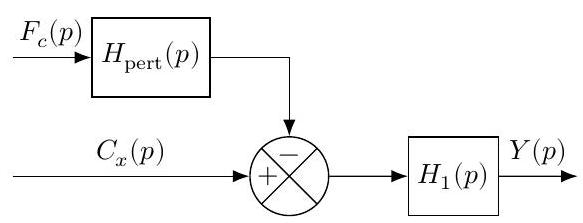
\includegraphics[width=.4\textwidth]{2023_07_26_54f5e859400a10e656ddg-07}
%Figure 10 
\caption{\label{fig:10}Schéma bloc du stabilisateur (1)}
\end{figure}

On rappelle que $L=0,3 \mathrm{~m}$ et les valeurs retenues pour $J_{x}, f$ et $k$ sont :

\begin{itemize}
  \item $J_{x}=1,14 \times 10^{-2} \mathrm{~kg} \cdot \mathrm{m}^{2}$;

  \item $-f=64 \times 10^{-3} \mathrm{~N} \cdot \mathrm{m} \cdot \mathrm{s} \cdot \mathrm{rad}^{-1}$;

  \item $-k=95 \mathrm{~N} \cdot \mathrm{m} \cdot \mathrm{rad}^{-1}$.
\end{itemize}

%Q 20. 
\question{\label{q:20}Écrire $H_{1}(p)$ sous forme canonique, puis calculer les valeurs de ses paramètres caractéristiques : gain statique $K_{1}$, amortissement $\xi_{1}$ et pulsation propre $\omega_{1}$. Commenter le comportement associé (fréquentiel ou temporel).}
\ifprof
\begin{corrige}
On a $H_1(p) = \dfrac{\dfrac{L}{k}}{1 + \dfrac{f}{k}p + \dfrac{J_x}{k}p^2}$, on identifie alors:
\begin{itemize}
\item[•] le gain statique $K_1 = \dfrac{L}{k} = \dfrac{0,3}{95} = 3,2\cdot 10^{-3}$rad/N;
\item[•] la pulsation propre $\omega_1 = \sqrt{\dfrac{k}{J_x}} = \sqrt{\dfrac{95}{1,14\cdot 10^{-2}}} = 91,3$rad/s;
\item[•] l'amortissement $\xi_1 = \dfrac{1}{2}\cdot \dfrac{f}{\sqrt{k J_x}} = \dfrac{1}{2}\cdot \dfrac{64\cdot 10^{-3}}{\sqrt{95 \times 1,14\cdot 10^{-2}}} = 0,03$. 
\end{itemize} 

On choisit de décrire le comportement dans le domaine fréquentiel. On a un système d'ordre 2 avec résonance (car $\xi_1 < \dfrac{\sqrt{2}}{2}$) à la pulsation $\omega_r = \omega_1\sqrt{1 - 2\xi_1^2}$. Le diagramme de Bode associé est le suivant:

\end{corrige}
\else
\fi


